% chktex-file -1
% chktex-file 24
% chktex-file 9
\chapter{Method}
\label{cha:method}

This chapter describes the theory used and developed in this thesis. First, the
notation for HMMs introduced in section~\ref{sec:hidden-markov-models} is
written out as this is used extensively in the following sections.

Next the classical Viterbi algorithm is described and it is described how it
may be reformulated to make use of the byte pair encoding and thereby gaining a
theoretical speedup.

The posterior decoding is then described, first the classical algorithm and
then the reformulated version. As this version does not obtain at speedup from
the byte pair encoding, theory for an \emph{indexed} posterior decoding
algorithm is given. This algorithm gains a theoretical speedup compared to the
classical formulation.

\section{Notation}

Recall the introduction to HMM's given in
section~\ref{sec:hidden-markov-models}. An HMM can generate an \emph{observed
  sequence} $Y_{1:T} = y_1y_2\dots{}y_T$ with $y_i \in \mathcal{O}$ by
traversing hidden states and emitting symbols. There exist one or more
\emph{paths} of hidden states $X_{1:T} = x_1x_2\dots{}x_T$ with
$x_i \in \mathcal{H}$ for each observed sequence generated by the HMM. Formally
a HMM is defined as
\begin{itemize}
\item $\mathcal{H} = {h_1, h_2, \dots, h_N}$, a finite alphabet of hidden
  states;
\item $\mathcal{O} = {o_1, o_2, \dots, o_M}$, a finite alphabet of observables;
\item a vector $\Pi = {(\pi_i)}_{1 \le i \le N}$, where $\pi_i = \Pr(x_1 =
  h_i)$ is the probability of the model starting in hidden state $h_i$;
\item a matrix $A = {\{a_{ij}\}}_{1 \le i \le N}$, where $a_{ij} = \Pr(x_t
  = h_j \mid x_{t - 1} = h_i)$ is the probability of a transition from state
  $h_i$ to state $h_j$;
\item a matrix $B = {\{b_{ij}\}}_{1 \le i \le N}^{1 \le j \le M}$, where
  $b_{ij} = \Pr(y_t = o_j \mid x_t = h_i)$ is the probability of state
  $h_i$ emitting $o_j$.
\end{itemize}
A HMM is parametrized by $\pi$, $A$, and $B$ and is denoted by $\lambda =
(\pi, A, B)$.

\section{The Classical Viterbi Algorithm}
\label{sec:class-viterbi-algor}

The Viterbi algorithm finds the probability of the most likely sequence of
hidden states given a model $\lambda$ and an observed sequence $Y_{1:T}$ by
maximizing the probability of the observed and hidden sequences for all
possible hidden sequences: $\Pr(Y_{1:T} \mid \lambda) = \max_{x_{1:T}}
\Pr(Y_{1:T}, X_{1:T} = x_{1:T} \mid \lambda)$. This may be computed efficiently
by filling out a table, $\omega$, with entries $\omega_t(x_t) = \Pr(Y_{1:t},
X_t = x_t \mid \lambda) = \max_{x_{1:t-1}} \Pr(Y_{1:t}, X_{1:t} = x_{1:t} \mid
\lambda)$ column by column from left to right, using the recursion
\begin{equation}
  \label{eq:1}
  \begin{aligned}
    \omega_1(x_1) &= \pi_{x_1} b_{x_1, y_1} \\
    \omega_t(x_t) &= b_{x_t, y_t} \max_{x_{t - 1}} \omega_{t - 1}(x_{t - 1})
    a_{x_{t - 1}, x_t}.
  \end{aligned}
\end{equation}
After filling out $\omega$, $\Pr(Y_{1:T} \mid \lambda)$ can be computed as
$\Pr(Y_{1:T} \mid \lambda) = \max_{x_T} \omega_T(x_T)$.

Note that only the last filled out column of $\omega$ needs to be stored, since
the recursion in equation~\eqref{eq:1} only needs the previous column to
compute the new one. Hence, the space consumption of the algorithm will be the
space needed for two columns and the input sequence, that is $O(N + T)$. To
fill out a cell in $\omega$ Viterbi maximizes over all cells in the previous
column resulting in a running time of $O\left(N^2 T \right)$.

\subsection{Backtracking}
\label{sec:backtracking-1}

To obtain the most likely sequence of hidden states corresponding to the
likelihood, $X_{1:T}^* = x_1^*, x_2^*, \dots, x_T^*$, also known as the
\emph{Viterbi path}, another table of the same size as $\omega$ is stored with
pointers from each state in a column to the maximizing previous state. When the
last column has been computed in $\omega$, the last state in the Viterbi path
may be found using $x_T^* = \argmax_{x_T} \omega_T(x_T)$. From this state the entire
path can be found by following the pointers in the table.

The space consumption of this backtracking algorithm is the size of $\omega$
which is $O(N T)$. Backtracking is done in $O(T)$ time using the table of pointers.

A space consumption of $O(N T)$ might be a problem in some scenarios. Another
way to backtrack is described by \citet{Tarnas01061998}. By using this approach
the space consumption can be reduced to $O\left(N \sqrt{T} \right)$ while the assymptotic
running time of the algorithm is preserved.

Instead of storing the entire $\omega$ table in memory only the last column of
blocks of some size $B$ is stored. These columns may be called checkpoints. A
table of pointers corresponding to a block can be recomputed using the
checkpoint of the previous block, since computing a column only requires the
previous block as seen in equation~(\ref{eq:1}). When backtracking $x_T^*$ may
be found as described above. The pointer tables are recomputed one at a time
for each block from right to left. When a table for a block has been recomputed
it is backtracked. Hence, only one block is kept in memory at a time. If
$B = \sqrt{T}$ is chosen, the space consumption of this algorithm is
$O\left(N \sqrt{T}\right)$. The Viterbi computations are now done two times, so the
algorithm will be a bit slower, but it keeps having the same assymptotic
running time of $O\left(N^2 T\right)$.

\section{Viterbi as Linear Algebra}
\label{sec:algorithm-as-linear}

In this chapter the theory of making the Viterbi algorithm faster by exploring
repetitions is discussed. First, the algorithm is reformulated into matrix
operations; second, the use of byte pair encoding is explained; and finally
a solution to make the computation numerically stable is explained.

The above classical Viterbi algorithm can be reformulated into a number of
matrix multiplications. This is what \citet{sand2013ziphmmlib} and
\citet{lifshits2009speeding} use too. First, let $B_{o_i}$ be the diagonal
matrix, having the emission probabilities of $o_i$ of the diagonal:
\begin{equation*}
  B_{o_i} =
  \begin{bmatrix}
    b_{1, o_i} &            &        &            \\
               & b_{2, o_i} &        &            \\
               &            & \cdots &            \\
               &            &        & b_{N, o_i} \\
  \end{bmatrix}
\end{equation*}
and let
\begin{align*}
  C_{o_i} &= B_{o_i} A^* \\
  C_1 &= B_{y_1} \pi,
\end{align*}
where $A^*$ is the transpose of $A$.

Now $\omega_t$ can be computed using $C_{y_t}$ and $\omega_{t - 1}$ as
\begin{equation}
  \label{eq:2}
  \omega_t = C_{y_t} \odot \omega_{t - 1} = C_{y_t} \odot C_{y_{t-1}} \odot
  \dots \odot C_1,
\end{equation}
where $\odot$ is the max-times matrix multiplication defined as ${(A \odot
  B)}_{ij} = \max_k A_{ik} \cdot B_{kj}$.

The classical Viterbi algorithm corresponds to computing this from right to
left. This will also be most efficient, since $C_1$ is a vector that when
multiplied by the matrix $C_2$ will result in a new vector. Hence, computing
$\omega_t$ from left to right will result in $t$ matrix-matrix multiplications,
while computing it from right to left will result in $t$ matrix-vector
multiplications that are more effecient to compute.

Backtracking is achieved in the same way as for the classical Viterbi algorithm
as described in section~\ref{sec:class-viterbi-algor}.

The space consumption and running time of this algorithm has changed, compared
to the classical Viterbi algorithm. For each symbol $o_i$ in the alphabet of
observables the corresponding matrix $B_{o_i}$ is created, thus requiring
$O\left(M N^2\right)$ space. The $C_{o_i}$ matrices require the same amount of space,
$O\left(M N^2\right)$. $C_1$ is vector, thus only requiring $O\left(N\right)$ space. If
equation~\eqref{eq:2} is evaluated from right to left it corresponds to a
series of matrix-vector multiplications resulting in a vector of size
$O\left(N\right)$. In total this requires $O\left(2 M N^2 + 2 N\right) = O\left(M N^2\right)$ space. If
backtracking is required the space consumption will be increased by the size of
the table of point that has size $O\left(N T\right)$. The total the space consumption with
backtracking enabled is $O\left(M N^2 + N T\right)$.

Likewise, the running time has changed. Creating the $B_{o_i}$ matrices takes
$O\left(M N^2\right)$ time. Computing the $C_{o_i}$ matrices takes time $O\left(M N^3\right)$ due to
the matrix multiplication. Computing $C_1$ takes $O\left(N^2\right)$ times. Again, if
equation~\eqref{eq:2} is evaluated from right to left, it will be matrix-vector
multiplication requiring $O\left(N^2 T\right)$ time. Backtracking can be done in $O\left(NT\right)$
time by using the table of pointers. In total this becomes $O\left(M N^2 + M N^3 +
N^2 + N^2 T + NT\right) = O\left(M N^3 + N^2 T\right)$.

\section{Exploiting Repetitions}
\label{sec:expl-repet}

In this section it is shown how to exploit repetitions in the observed sequence
to make the above algorithm run faster. \citet{lifshits2009speeding} introduces
five different methods of doing this, while \citet{sand2013ziphmmlib} only uses
byte-pair encoding.

\subsection{Byte-Pair Encoding}

Byte-pair encoding is a simple data compression method. The most common pair
consecutive bytes in the data is replaced by a byte that do not exist in the
data. This is repeated until either all new bytes are used or the most common
pair do not appear frequently in the data. The use of bytes may easily be
replaced by used of characters or intergers. For example, the input sequence
01012012 would first be encoded into 33232 by substituting 01 with 3; in the
next iteration it would be encoded into 344 by substituding 32 by 4 etc.

\subsection{Using Byte-Pair Encoding to Speed Up Viterbi}
\label{sec:using-byte-pair}

The Viterbi algorithm achieves a speed up using byte-pair encoding in the
following way. Let $o_i o_j \in O \times O$ be the most frequently occuring
pair of symbols in $Y_{1:T}$ and let $n_{o_i o_j}$ be the number of
occurences. $o_i o_j$ is substituded by a new symbol $o_{M + 1}$ and the length
of $Y_{1:T}$ is thereby reduced by $n_{o_i o_j}$. All $n_{o_i o_j}$ occurences
of $C_{o_i} \odot C_{o_j}$ in equation~\eqref{eq:2} may be replaced by the new
matrix
\begin{equation}
  \label{eq:7}
  C_{o_{M + 1}} = C_{o_i} \odot C_{o_j}.
\end{equation}
Hence, the number of matrix multiplications is reduced by $n_{o_i o_j}$. The
byte-pair encoding continues until $n_{o_i o_j}$ becomes too small to give a
speed up. This is discussed later. The result of this is a new sequence
$Y_{1:T'}'$ over the new alphabet
$\mathcal{O}' = \{o_1, o_2, \dots, o_M, o_{M + 1} = (l_1, r_1), o_{M + 2} =
(l_2, r_2), \dots, o_{M'} = (l_{M' - M}, r_{M' - M}) \}$,
where $l_i, r_i \in \{ o_1, o_2, \dots, o_{i - 1} \}$.

This method can be split up into two separate computations. First the
preprocessing consisting the of encoding the sequence as just discussed is
done. As the encoding of the sequence is independent of the HMM the encoded
sequence may be saved to the disk for later use. The second part consist of the
actual Viterbi algorithm and can be split into two stages. The first stage is
the computation of $C_{o_i}$ for $i = 1, \dots, M$ and then $C_{o_i}$ for
increasing $i = M + 1, \dots, M'$ by $C_{o_i} = C_{l_i} \odot C_{l_r}$. In the
second stage $\omega_T$ is computed by
\begin{equation}
  \label{eq:3}
  \omega_T = C_{y'_{T'}} \odot C_{y'_{T'-1}} \odot \dots \odot C_{y'_2} \odot C_1.
\end{equation}

A illustration of this method is given in
figure~\ref{fig:exploiting-repetitions}. As seen, when the computation has
finished, only a subset of the columns of $\alpha$ is computed.

\begin{figure}
  \centering
  Figure from \citet{sand2013ziphmmlib} here. Also draw the columns that are
  not computed.
  \caption{Exploiting repetitions in the observed sequence to speed up the
    Viterbi algorithm.}
  \label{fig:exploiting-repetitions}
\end{figure}

\subsection{Backtracking}
\label{sec:backtracking}

Obtaining the Viterbi path $S = s_1, s_2, \dots, s_T$ of $Y_{1:T}$ is no longer
as simple as for the classical Viterbi algorithm. Using the standard
backtracking methods, only the Viterbi path $S' = s_1', s_2', \dots, s_{T'}'$
of the compressed sequence $Y'_{1:T'}$ may be found. The path corresponds to
the columns in figure~\ref{fig:exploiting-repetitions} that have been
computed. It turns out that $S$ can be inferred from $S'$ since $S'$
is a subsequence of $S$ as described by \citet{lifshits2009speeding}. To do
this a set of matrices $R_{o_i}$ is kept along the $C_{o_i}$ matrices for each
of the new symbols $o_{M + 1}, \dots, o_{M' - M}$ defined as
\begin{equation*}
  R_{o_{M + i}}(m, n) = \argmax_k
  \left(
    C_{l_i}(m, k) \odot C_{r_i}(k, n)
  \right).
\end{equation*}
This is looks like the definition of the $C_{o_i}$ matrices from
equation~\eqref{eq:7}, but instead of storing the maximum value, the state that
results in the maximum value is stored.

Now, for each occurence of a new symbol $o_{M + i} = (l_i, r_i)$ where
$l_i, r_i \in \mathcal{O}$ in $Y_{1:T'}'$ we know the start state $s_l$ and the
end state $s_r$ from $S'$, such that $s_l$ is the state immediatly before $l_i$
was emitted and $s_r$ is the state after $r_i$ was emitted. Hence, we need to
find the most likely state where $l_i$ is emitted. This state is easily
obtained since it is stored at $R_{o_{M + i}}(s_l, s_r)$. In the case where one
or both of $l_i, r_i \not \in \mathcal{O}$ we can apply this method
recursively to obtain $S$.

This is illustrated in figure~\ref{fig:infering-viterbi-path}.

\begin{figure}
  \centering
  Figure 3 here.
  \caption{Infering the Viterbi path $S_T$ from the partial path $S_{T'}'$.}
  \label{fig:infering-viterbi-path}
\end{figure}

Since $S'$ may be found in two different ways as discussed in
section~\ref{sec:backtracking-1}, three different variations of the Viterbi
algorithm may be defined.
\begin{description}
\item[Viterbi\textsubscript{L}] that compresses the sequence and only computes the
  loglikelihood,
\item[Viterbi\textsubscript{P}] that also backtracks using a table of pointers,
\item[Viterbi\textsubscript{PM}] that saves memory on backtracking by using checkpoints.
\end{description}
The same variations may be defined for the classical Viterbi algorithm.

\subsection{Running Time}
\label{sec:running-time}

The space consumption is comparable to the Viterbi algorithm without
compression enabled. The number of $C$ matrices has changed from $M$ to $M'$
thus requiring $O\left(M' N^2\right)$ space. The introduction of the $R$ matrices does not
change this since the $C$ matrices are of similar size. The table used for the
simple backtracking has decreased to size $O\left(N T'\right)$. The Viterbi path has size
$T$ resulting in a total space consumption of $O\left(M' N^2 + N T' + T\right)$ for
Viterbi\textsubscript{P}. For Viterbi\textsubscript{PM} the space consumption will be
$O\left(M' N^2 + N \sqrt{T'} + T\right)$.

With similar arguments the running time of computing the likelihood has changed
to $O\left(M' N^3 +N^2 T'\right)$. Using the the the $R$ matrices the Viterbi path can be
obtained in $O\left(N^2 T' + T\right)$ time. Hence, the running time with backtracking
enabled is $O\left(M' N^3 +N^2 T' + T\right)$.

The running time of the preprocessing part is $O\left(
\left(
  \lvert\mathcal{O'}\rvert - \lvert{\mathcal{O}}\rvert
\right) T\right)$, since one new symbol is introduced by scanning the input sequence for
pairs. Note that the $\lvert\mathcal{O'}\rvert - \lvert{\mathcal{O}}\rvert$
factor depends on the input. For sequences with many repetitions the byte-pair
encoding will continue for more iterations than for sequences with few
repetitions.

An overview of the theoretical running times and space consumptions is shown in
table~\ref{tab:running-time}.

\begin{table}
  \centering
  \caption{Running time and space consumption of the different variations of the
    Viterbi algorithm.}
  \label{tab:running-time}
  \begin{tabular}{lll}
    \toprule
    Algorithm                   & Running time             & Space consumption             \\
    \midrule
    Classical\textsubscript{L}  & $O\left(N^2 T\right)$               & $O\left(N + T\right)$                    \\
    Classical\textsubscript{P}  & $O\left(N^2 T\right)$               & $O\left(NT\right)$                       \\
    Classical\textsubscript{PM} & $O\left(N^2 T\right)$               & $O\left(N\sqrt{T}\right)$                \\
    Viterbi\textsubscript{L}    & $O\left(M' N^3 + N^2 T'\right)$     & $O\left(M' N^2 + T'\right)$              \\
    Viterbi\textsubscript{P}    & $O\left(M' N^3 + N^2 T' + T\right)$ & $O\left(M' N^2 + N T' + T\right)$        \\
    Viterbi\textsubscript{PM}   & $O\left(M' N^3 + N^2 T' + T\right)$ & $O\left(M' N^2 + N \sqrt{T'} + T\right)$ \\
    \bottomrule
  \end{tabular}
\end{table}

\subsection{Saving Compressed Sequence and Computed Matrices}
\label{sec:saving-compr-sequ}

As mentioned the sequence encoding is independent of the HMM and may be saved
for use with different HMMs. This makes it possible to compress the sequence
once and then make use of the compressed sequence multiple times with different
HMMs. \citet{lifshits2009speeding} also suggests constructing the substitution
table for the compression based on a set of representative sequences. Then the
$C_{o_i}$ matrices could be computed beforehand and also saved to the
disk. This is useful if many sequences are used with one HMM.\

\subsection{Numerical Stability}

All matrices contain probabilities, i.e.\ the are in range between 0 and
1. Multiplying them together results in even smaller numbers. Since the value
is stored as a IEEE 754 floating point format there is a limited precission,
and the computations will quickly underflow. \citet{sand2013ziphmmlib}
describes how to avoid underflow in terms to the forward algorithm. It turns
out that it is easier to avoid for the Viterbi algorithm.

To circumvent underflow in the classical Viterbi algorithm all probabilities
are converted to log-space. So, instead of computing $\omega_T$,
$\log \omega_T$ is computed. By using the the property that
$\log(AB) = \log A + \log B$ the multiplications are turned into additions,
which makes the algorithm much more stable to underflow.

The same idea can be used for the matrix based approach, where
equation~\eqref{eq:3} is rewritten as
\begin{align*}
  \log \omega_T &= \log \left(C_{y'_{T'}} \odot C_{y'_{T'-1}} \odot \dots \odot
                  C_{y'_2} \odot C_1 \right) \\
                &= \log C_{y'_{T'}} \oplus \log C_{y'_{T'-1}} \oplus \dots \oplus
                  \log C_{y'_2} \oplus \log C_1,
\end{align*}
and the $C$ matrices are rewritten as
\begin{align*}
  C_1 &= \log B_{y_1} \pi, \\
  C_{o_i} &= \log B_{o_i} A^*, \quad \text{for }1 \le i \le M\\
  C_{o_{M + i}} &= C_{l_i} \oplus C_{r_i} , \quad \text{for }1 \le i \le M' - M
\end{align*}
where $\oplus$ is defined as
${ \left( A \oplus B \right)}_{ij} = \max_k \left( \log A_{ik} + \log B_{kj}
\right)$.


\subsection{Compression Stopping Criterion}
\label{sec:compr-stopp-crit}

Using the byte-pair compression method a sequence can be compressed until only
a single character is present. However, as more symbols are added to the
alphabet, the most common pair of symbols will be less and less frequent as the
sequence gets more compressed. This means that the first iterations of the
compression will make the sequence much shorter whereas the later iterations
will not compress the sequence as effectively as the first. Hence, for the
first iterations of the compression, a large increase in the speedup of Viterbi
is expected, where the increase in speedup of later iterations will be more
modest.

\citet{sand2013ziphmmlib} describe a method on how to determine when the
compression should stop for the forward algorithm. The user of the program
supplies an estimate $e$ of how many times the compressed sequence is going to
be used. For a low $e$ the algorithm should not spend too much time on
compressing the sequence while for a high value of $e$, the algorithm can
``afford'' spending more time on compression, since the time spent will be
reearned again when running the actual algorithm.

Furthermore the user specifies a parameter $N_{\text{min}}$ that is the number
of states in the model that will be used. In the compression phaze it is
estimated how much time will be spent on the actual $e$ executions of the
actual algorithm, by measuring the time it takes to do a matrix-matrix
multiplication and a matrix-vector multiplication with matrices of size
$N_{\text{min}}$. Hence, it may be estimated how long it will take to execute
the actual algorithm. When the time it takes to make another iteration of the
compression is larger than the estimate of the time saved in the execution of
the algorithm, the compression is stopped. If a single value of
$N_{\text{min}}$ cannot be found a list of parameters
$(N_{\text{min}}^1, N_{\text{min}}^2, \dots)$ may be specified and the input
sequence will be compressed for each of these model sizes. If no
$N_{\text{min}}$ parameter is provided the compression continues until the
frequency of the most common pair is the same in two consequtive iterations.

This method may be reused for the Viterbi algorithm. Instead of measuring the
time it takes to do matrix-matrix multiplications and matrix-vector
multiplications, the time measured for max-times multiplications is used.

This simple algorithm does not take backtracking into account, since the time
estimated is only for the computation of the likelihood. By letting the user
specify whether backtracking is required, the time estimation could also
involve an estimate on how much time will be spent on backtracking, by
estimating the time it takes to allocate an array of size $T$ and
infer the Viterbi path $S$ from the compressed path $S'$. This has
not been implemented.

\section{Classical Posterior Decoding}
\label{sec:posterior-decoding-1}

The Viterbi algorithm described above find the most likely path of hidden
states through the HMM emitting the input sequence. Another kind of decoding is
called posterior decoding. Posterior decoding finds the most likely state at
the time the symbol is emitted. Formally the most likely state
$s_t \in \mathcal{H}$ being in when emitting symbol $y_t$ may be written as
\fxwarning{Rename $s_t$ to something else to avoid confusion with Viterbi
  path?}
\begin{equation*}
  s_t = \argmax_{x_t \in \mathcal{H}} \Pr \left(x_t | Y_{1:T}, \lambda \right).
\end{equation*}
The posterior decoding $X_{1:T}$ is a sequence of hidden states that might not
be a valid path according to the transitions of the model, like the Viterbi
decoding, but it may still be useful for some applications.

The posterior decoding may be efficiently computed using the forward-backward
algorithms. The forward-backward algorithms are comparible to the Viterbi
algorithm. Instead of computing the probability of most likely path, they
compute the joint probability of all paths, that is
\begin{equation*}
  \Pr
  \left(
    Y_{1:T} \mid \lambda
  \right) = \sum_{x_{1:T}} \Pr
  \left(
    Y_{1:T}, X_{1:T} = x_{1:T} \mid \lambda
  \right).
\end{equation*}

For the classical forward algorithm a table, $\alpha$, with entries
\begin{equation*}
\alpha_t(x_t) = \Pr \left( Y_{1:t}, X_t = x_t \mid \lambda \right) =
\sum_{x_{1:t-1}} \Pr \left( Y_{1:t}, X_{1:t} = x_{1:t} \mid \lambda \right)
\end{equation*}
is filled. As seen this is very similar to the Viterbi algorithm. Instead of
taking the maximum over all previous states the sum is computed. Computing
$\alpha$ may be done recursively column by column from left to right like the
Viterbi algorithm using
\begin{equation}
  \label{eq:8}
  \begin{aligned}
    \alpha_1(x_1) &= \pi_{x_1} b_{x_1, y_1} \\
    \alpha_t(x_t) &= b_{x_t, y_t} \sum_{x_{t - 1}} \alpha_{t - 1}(x_{t - 1})
    a_{x_{t - 1}, x_t}.
  \end{aligned}
\end{equation}

Where the forward algorithm computes the table from left to right, i.e.\
it computes the joint probability of emitting $y_t$ after having emitted
$y_{1:t-1}$, the backward algorithm computes the joint probability of emmiting
$y_t$ and then emitting $y_{t+1:T}$. This corresponds to filling the table from
right to left. The backward table is called $\beta$. The recursion may be written as
\begin{equation}
  \label{eq:9}
  \begin{aligned}
    \beta_T(x_T) &= (1, 1, \dots, 1) \\
    \beta_t(x_t) &= b_{x_t, y_t} \sum_{x_{t + 1}} \beta_{t + 1}(x_{t + 1})
    a_{x_{t + 1}, x_t}.
  \end{aligned}
\end{equation}
The rightmost column is filled with 1's, since the initial state is assumed
given.

After having computed the forward and backward tables, it is now possible to
compute the posterior decoding $S_{1:T}$ given by
\begin{equation*}
  s_t = \argmax_{x_t \in \mathcal{H}} \Pr \left(x_t \mid Y_{1:T} \right) =
  \argmax_{x_t \in \mathcal{H}} \frac{\alpha(x_t) \beta(x_t)}{\Pr \left( Y_{1:T} \right)}.
\end{equation*}
Since $\Pr \left( Y_{1:T} \right)$ is the same for all $t$ it may be treated as
a constant result in the formula
\begin{equation}
  \label{eq:6}
  s_t = \argmax_{x_t \in \mathcal{H}} \alpha(x_t) \beta(x_t).
\end{equation}

\section{Posterior Decoding as Linear Algebra}

The main part of the posterior decoding algorithm described in the previous
section is computing the forward and backward tables. Once this is done it is
easy to compute the posterior decoding. The forward and backward algorithms may
be expressed as linear algebra similarly to the Viterbi algorithm.

The theory, implementation of, and experimentation with the forward algorithm
is done by \citet{sand2013ziphmmlib}. As the theory described in
section~\ref{sec:algorithm-as-linear} is built upon and using the same notation
as work done by \citet{sand2013ziphmmlib} the description of the forward
algorithm is omitted in this thesis.

Expressing the backward algorithm in terms of matrix multiplications is
essentially the same as the forward algorithm as the two algorithms are very
similar as seen in section~\ref{sec:posterior-decoding-1}. Let the emission
matrices, $B_{o_i}$, matrices be identical to the ones described in
section~\ref{sec:algorithm-as-linear}. We can then set the $C$ matrices to
\begin{equation}
  \label{eq:4}
  \begin{aligned}
    C_{o_i} & = B_{o_i} A^*, \\
    C_T & = (1, 1, \dots, 1).
  \end{aligned}
\end{equation}
Now $\beta_t$ can be computed using $C_{y_t}$ and $\beta_{t + 1}$ as
\begin{equation}
  \label{eq:5}
  \begin{aligned}
    \beta_t = C_{y_t} \beta_{t - 1} = C_{y_t} C_{y_{t+1}}\dots C_T,
  \end{aligned}
\end{equation}
which is similar to the forward algorithm in \citet{sand2013ziphmmlib} and the
Viterbi algorithm in section~\ref{sec:algorithm-as-linear}, except that the
matrix multiplications no longer are max times multiplications but normal
matrix multiplications.

The assymptotic running time and space consumption is equal to the running time
and space consumption of the Viterbi algorithm.

\fxerror{Describe that the same approach as for classical posterior decoding is used.}

\subsection{Numerical Stability}

Like for the the Viterbi algorithm a lot of probabilities are multiplied and
numerical issues will occur. For the Viterbi algorithm this was solved by
working in logarithmic space.

\citet{sand2013ziphmmlib} describes how to make the computations in the forward
algorithm numerically stable. First, as the $C$ matrices in
equation~\eqref{eq:4} are defined by matrix multiplications, they tend to
underflow, since each matrix consists of entries in the interval $[0, 1]$. To
overcome this problem in for forward algorithm the matrices are normalized,
that is they are scaled by the sum of the entries in the matrix. This may be
reused in the backward algorithm as well, as the $C$ matrices are computed in
the same way.

For the computation of the forward table, $\alpha$, the columns underflow when
$T$ gets large, since the computation is defined by multiplications of
probabilities. A similar approach is used to overcome this problem. Each column
is normalized by scaling with the sum of the entries. This makes the forward
table computation numerically stable. Since the magnitudes of the entries in
the forward table and backward table entries are comparable, it is reasonable
to use the scalars from the forward table in the computation of the backward
table in equation~\eqref{eq:5}. Using the same scalars is also required for the
result in equation~\eqref{eq:6} to be correct, since the use of different
scalars for columns in the forward and backward tables could give arbitrary
results.



\section{Problems in Exploiting Repetitions}
\label{sec:probl-expl-repet}

\citet{sand2013ziphmmlib} exploits repetitions for the forward algorithm using
byte-pair encoding similarly to the description in
section~\ref{sec:expl-repet} but do implement any kind of backtracking. Using
the same method it is easy to also exploit repetetions in the backward
algorithm.

To compute the posterior decoding of the uncompressed sequence from the
forward and backward tables of the compressed sequence, either (1) the
posterior decoding sequence may be computed using the partial path obtained
from the compressed sequence, or (2) the entire forward and backward tables of
the uncompressed sequence are required. For both approaches the running time of
computing 1 state in the posterior decoding must take strictly less than
$O\left(N^2\right)$ time to gain a speedup, since one else might as well compute the
forward and backward tables without compressing the input sequence. The two
approaches are now discussed in turn.

\begin{enumerate}
\item For the Viterbi algorithm it is in section~\ref{sec:backtracking}
  described how the $R$ matriced can be precomputed to retrieve the full
  Viterbi path from the partial path. This method makes use of the property
  that the Viterbi algorithm maximizes over all previous states. From the
  partial path the previous state that maximizes the likelihood is known. Using
  this information the current state may be found using only $O\left(N\right)$ time, since
  it is not necessary to maximize over all previous states. Using information
  about the next state it is possible to precompute the maximizing state for
  each symbol for all previous and all next states, and thus computing the
  current state in constant time.

  The problem is that for the forward-backward algorithm the current state do
  not only depend on the previous state, since it is not computed using the
  maximum over all previous states but the sum of these. Hence, having computed
  the partial path does not help retrieving the full path as the full path is
  not dependent on partial path.
\item Computing the full forward and backward tables is another approach. Since
  the full tables have have $N$ entries in each column the running time of
  filling an entry must take strictly less than $O\left(N\right)$ time to gain a
  speedup. It might be possible that some relation exist between missing
  columns in the partial tables that corresponds to the same symbol in the
  input sequence.

  Looking at figure~\ref{fig:full-forward-table}, assume the columns $i$ and
  $j$ has been computed using the compressed sequence. The columns $i + 1$ and
  $j + 1$  that correspond to the same symbol needs to be computed. It is an
  open question whether it is posible to compute those faster than the naïve
  approach that takes $2N^2$ time.
\end{enumerate}

\begin{figure}
  \centering
  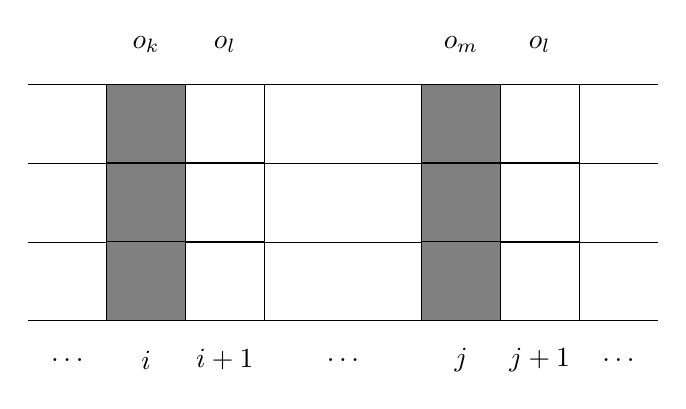
\begin{tikzpicture}
  \tikzstyle{box} = [draw=black, minimum width=10mm, minimum height=10mm];
  \tikzstyle{gray_box}  = [box, fill=gray];
  \tikzstyle{white_box} = [box];


  \draw[very thin] (-1.5, -0.5) -- (6.5, -0.5);
  \draw[very thin] (-1.5, 0.5)  -- (6.5, 0.5);
  \draw[very thin] (-1.5, 1.5)  -- (6.5, 1.5);
  \draw[very thin] (-1.5, 2.5)  -- (6.5, 2.5);

  \node[gray_box]  at (0, 0) {};
  \node[white_box] at (1, 0) {};
  \node[gray_box]  at (4, 0) {};
  \node[white_box] at (5, 0) {};

  \node[gray_box]  at (0, 1) {};
  \node[white_box] at (1, 1) {};
  \node[gray_box]  at (4, 1) {};
  \node[white_box] at (5, 1) {};

  \node[gray_box]  at (0, 2) {};
  \node[white_box] at (1, 2) {};
  \node[gray_box]  at (4, 2) {};
  \node[white_box] at (5, 2) {};

  \node at (0, 3) {$o_k$};
  \node at (1, 3) {$o_l$};
  \node at (4, 3) {$o_m$};
  \node at (5, 3) {$o_l$};

  \node at (-1, -1) { $\dots$};
  \node at (0, -1)  { $i$};
  \node at (1, -1)  { $i+1$};
  \node at (2.5, -1)  { $\dots$};
  \node at (4, -1)  { $j$};
  \node at (5, -1)  { $j+1$};
  \node at (6, -1)  { $\dots$};
\end{tikzpicture}
%%% Local Variables:
%%% mode: latex
%%% TeX-master: "../master"
%%% End:

  \caption{Computing the full forward table from the partial table. Note that
    in figures~\ref{fig:exploiting-repetitions}
    and~\ref{fig:infering-viterbi-path} where the sequence was written from
    right to left, i.e.\ the indices were increasing from right to left. In
    this illustration the indicies in this illustration are increasing from
    left to right, since it is more natural to think about. The gray boxes
    indicate columns filled during the when computing the table for the
    compressed sequence. The white columns needs to be computed in less than
    $O\left(N^2\right)$ time per column.}
  \label{fig:full-forward-table}
\end{figure}

Unfortunately no solution to this problem has been found. Hence, the posterior
decoding cannot be speeded up by exploiting repetitions in the observed
sequence. The running time of computing the posterior decoding is then
$O\left(M N^3 + TN^2\right)$, which is assymptotically worse than the classical posterior
decoding algorithm that runs in $O\left(TN^2\right)$. Note though that the alphabet size
$M$ typically is small, so it is expected that the assymptotic running times of
the two algorithms in practice are comparable.

\section{Indexed Posterior Decoding}

In the last section it was discussed that the posterior decoding for an
observed sequence cannot be done assymptotically faster using the byte-pair
compression. However, if only parts of the posterior decoding are needed
instead of the entire path, a speedup may be obtained.

For indexed posterior decoding not only an input sequence $Y_{1:T}$ and a model
$\lambda$ is given as input, but also two indexes $i,j \in [1:T]$. Instead of
returning the posterior decoding $X_{1:T}$ the only the part of the sequence
from index $i$ to $j$ denoted $X_{i:j}$ is returned.

Recall from section~\ref{sec:using-byte-pair} that the columns of the forward
and backward tables, $\alpha'$ and $\beta'$, of the compressed sequence
$Y_{1:T'}'$ are a subset of columns in the tables, $\alpha$ and $\beta$, of
$Y_{1:T}$. Furthermore, recall that a column may be computed using the column
emmediately to the left or right for the forward and backward algorithms
respectively as seen in equation~\eqref{eq:8} and~\eqref{eq:9}. Using this, the
columns $i$ to $j$ of the forward and backward tables, $\alpha$ and $\beta$,
corresponding to the \emph{subsequence} $Y_{i:j}$ may be found using existing
columns from the forward and backward tables, $\alpha'$ and $\beta'$.

\begin{figure}
  \centering
  \tikzsetnextfilename{subsequence_posterior}
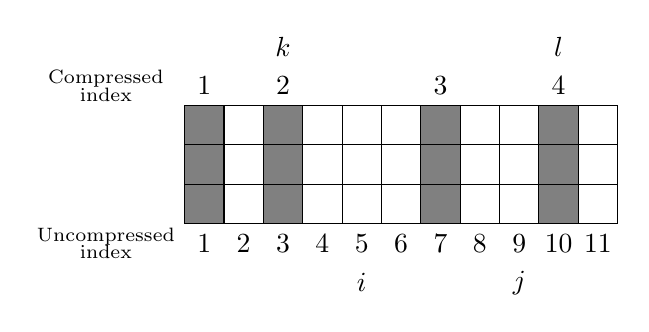
\begin{tikzpicture}
  [scale=0.5]
  \tikzstyle{box} = [draw=black, minimum width=5mm, minimum height=5mm];
  \tikzstyle{gray_box}  = [box, fill=gray];
  \tikzstyle{white_box} = [box];


  \node at (2, 4) {$k$};
  \node at (9, 4) {$l$};

  \node[gray_box]  at (0, 0) {};
  \node[gray_box]  at (0, 1) {};
  \node[gray_box]  at (0, 2) {};

  \node[white_box]  at (1, 0) {};
  \node[white_box]  at (1, 1) {};
  \node[white_box]  at (1, 2) {};

  \node[gray_box]  at (2, 0) {};
  \node[gray_box]  at (2, 1) {};
  \node[gray_box]  at (2, 2) {};

  \node[white_box]  at (3, 0) {};
  \node[white_box]  at (3, 1) {};
  \node[white_box]  at (3, 2) {};

  \node[white_box]  at (4, 0) {};
  \node[white_box]  at (4, 1) {};
  \node[white_box]  at (4, 2) {};

  \node[white_box]  at (5, 0) {};
  \node[white_box]  at (5, 1) {};
  \node[white_box]  at (5, 2) {};

  \node[gray_box]  at (6, 0) {};
  \node[gray_box]  at (6, 1) {};
  \node[gray_box]  at (6, 2) {};

  \node[white_box]  at (7, 0) {};
  \node[white_box]  at (7, 1) {};
  \node[white_box]  at (7, 2) {};

  \node[white_box]  at (8, 0) {};
  \node[white_box]  at (8, 1) {};
  \node[white_box]  at (8, 2) {};

  \node[gray_box]  at (9, 0) {};
  \node[gray_box]  at (9, 1) {};
  \node[gray_box]  at (9, 2) {};

  \node[white_box]  at (10, 0) {};
  \node[white_box]  at (10, 1) {};
  \node[white_box]  at (10, 2) {};

  \node[align=center] at (-2.5, 3) {\scriptsize Compressed \\[-2mm] \scriptsize index};

  \node at (0, 3) {1};
  \node at (2, 3) {2};
  \node at (6, 3) {3};
  \node at (9, 3) {4};

  \node[align=center] at (-2.5, -1) {\scriptsize Uncompressed \\[-2mm] \scriptsize index};

  \node at (0, -1) {1};
  \node at (1, -1) {2};
  \node at (2, -1) {3};
  \node at (3, -1) {4};
  \node at (4, -1) {5};
  \node at (5, -1) {6};
  \node at (6, -1) {7};
  \node at (7, -1) {8};
  \node at (8, -1) {9};
  \node at (9, -1) {10};
  \node at (10, -1) {11};

  \node at (4, -2) {$i$};
  \node at (8, -2) {$j$};

\end{tikzpicture}
%%% Local Variables:
%%% mode: latex
%%% TeX-master: "../master"
%%% End:

  \caption{Illustration of the computation of the forward (or backward) table
    for a substring of the uncompressed sequence given by indices $i$ to $j$,
    given that the columns of the forward table for the compressed sequence,
    shown in grey, have been computed in advance.}
  \label{fig:subsequence-posterior}
\end{figure}

An example of the above is illustrated in
figure~\ref{fig:subsequence-posterior}. Assume that the forward table $\alpha'$
and the backward table $\beta'$ for the compressed sequence has been computed.
This is shown as grey columns. To compute $\alpha$ and $\beta$ from index $i$
to $j$, the computed column at some index $k$ with $k \le i$ may be used as a
starting point for the forward computation. In this example that is index 3
that corresponds to the column at index 2 in $\alpha'$. Likewise, some column
$l$ with $l \ge j$ can be used as a starting point for the
computation of the backward table.

\subsubsection{Starting Point Columns}

To find the indicies $k$ and $l$ for the uncompressed sequence and the
corresponding indicies $k'$ and $l'$ for the compressed sequence, a sorted
mapping \texttt{orig\_index2comp\_index} from uncompressed indices to
compressed indices is created. In this example the map would consist of the
mappings $1 \rightarrow 1, 3 \rightarrow 2, 7 \rightarrow 3$ and
$10 \rightarrow 4$. To find the index $k$, a binary search is performed on the
map to find the largest key less than or equal to $i$. The value corresponding
to $k$ is $k'$. Likewise $l$ and $l'$ may be found by finding the smallest key
larger than or equal to $j$.

To compute this mapping, another mapping \texttt{symbol2length} from each
symbol in the new alphabet $\mathcal{O'}$ to its original length is
created. This may be done iteratively by inserting first inserting each
original symbol $o_1, \dots, o_M \in \mathcal{O}$ with length 1 into the
map. Next, $o_{M+1}, o_{M+2}, \dots, o_{M'} \in \mathcal{O'}$ is inserted in
the specified order. As each new symbol $o_c \in \mathcal{O'}$ is created using
two existing symbols $o_a$ and $o_b$ the length of $o_c$ can be computed by
using the map to get the the lengths of $o_a$ and $o_b$ and add these two
together.

Now \texttt{orig\_index2comp\_index} is computed by scanning through the
compressed sequence one symbol at a time while incrementing the corresponding
index in the uncompressed sequence by using the map of lengths.

The starting columns for the forward and backward algorithms have now been
found. The only thing missing for the computation is the sequence for which to
compute the following (for forward) or preceding (for backward) columns.

\subsubsection{Sequence}

The simplest solution for finding a sequence for which to compute the forward
and backward tables is to store the original sequence $Y_{1:T}$ and then
extract the sequence $Y_{k:l}$ from that. Instead of storing $Y_{1:T}$,
$Y_{k:l}$ may be found by decompressing $Y_{k':l'}'$. This may be done by
replacing the symbols $o_{M + 1}, \dots, o_{M'}$ by symbols from the original
alphabet $\mathcal{O}$. An example of this algorithm is shown in
algorithm~\ref{alg:simple-decompress}. The $\alpha$ and $\beta$ tables may be
found by computing the columns corresponding to $Y_{k:l}$ and afterwards remove
columns $[k, i)$ and $(l, n]$.

\begin{algorithm}
  \caption{Simple decompression algorithm.}
  \label{alg:simple-decompress}
  \begin{algorithmic}[1]
    \Procedure{decompress\_substring}{$Y', i, j, k, l, k', l'$}
        \State{String $Z \gets Y_{k':l'}'$}
        \For{$c = M'$ \textbf{down to} $M + 1$}
          \State{$o_l, o_r \gets $ get\_pair($o_c$)}
          \State{Replace $o_c$ by $o_{l}o_{r}$ in $Z$}
        \EndFor{}
        \State{\Return{$Z$}}
    \EndProcedure{}
  \end{algorithmic}
\end{algorithm}

Decompressing $Y_{k':l'}'$ entirely might be inefficient though. If the
compressed sequence $Y_{1:T'}'$ is much compressed, i.e.\ $T' \ll T$, the
length of $Y_{k:l}$ may be much larger than $Y_{i:j}$. In the worst case of
$T' = 1$, the decompression would result in the uncompressed sequence
$Y_{1:T}$. Hence, the indexed posterior decoding algorithm will spend a lot of
time computing columns that is thrown away afterwards, and the running time is
$O\left(M' N^3 + N^2 T\right)$ which is not an improvement over the classical
posterior decoding. The decompression needs to be made smarter.

Observe that only the symbols from index $[i,j]$ needs to be from the orignal
alphabet $\mathcal{O}$. The symbols from $[k, i)$ and $(j, l]$ may be from the
new alphabet, since each column in the these parts of $\alpha$ and $\beta$ are
not needed for the posterior decoding computation. Hence, when decompressing
$Y_{k':l'}'$ symbols that correspond to uncompressed symbols in the interval
$[k, i)$ should not be decompressed and left as compressed symbols. Likewise,
symbols corresponding to the interval $(j, l]$ should not be decompressed. As
before, symbols corresponding to uncompressed symbols that overlap $[i, j]$
should be decompressed. If this is done, the partial decompression of
$Y_{k':l'}'$ resulting in a new sequence $Z$ will then contain some symbols
from $\mathcal{O'}$ at the beginning, then some symbols from $\mathcal{O}$ in
the middle being the symbols $Y_{i:j}$, and then some symbols from
$\mathcal{O'}$ again in the end.

An algorithm for doing this takes as input a compressed sequence $Y'$ and the
indicies $i, j, k, l, k'$ and $l'$. The symbols of substring $Y_{k':l'}'$ is
pushed to a stack $Y^S$, such that $Y_{l'}'$ is at the bottom and $Y_{k'}'$ at
the top. The algorithm pops symbols one by one from $Y^S$, while the
corresponding index into the uncompressed sequence $Y$ is maintained by using
the \texttt{symbol2length} map. When a symbol $c$ that overlap $[i, j]$ is
encountered $c$ is either appended to $Z$ if $c \in \mathcal{O}$ or it is split
into a pair and pushed to of $Y^S$, such that the left symbol of that pair will
be popped in the next iteration. The first time a symbol $c \in \mathcal{O}$
overlaps $[i, j]$ is encountered, the index (named \texttt{start\_index}) of
that symbol in $Z$ is saved, as it is used later for computing the posterior
decoding. If $c$ overlaps $[k, l]$ it is appended to $Z$. In case there is no
overlap between $c$ and $[k, l]$ nothing is done, i.e.\ $c$ is thrown away.
Pseudo code for this algorithm is given in algorithm~\ref{alg:decompress}. This
algorithm is much more effecient to use for very compressed sequences.

\begin{algorithm}
  \caption{Partially decompress the compressed sequence.}
  \label{alg:decompress}
  \begin{algorithmic}[1]
    \Procedure{decompress\_substring}{$Y', i, j, k, l, k', l'$}
        \State{String $Z \gets $ nil}
        \State{Stack $Y^S \gets $ nil}
        \State{Push $Y_{l'}', \dots, Y_{k'}'$ to $Y^S$}
        \State{start\_index $\gets$ nil}
        \State{index $\gets k - (\text{symbol2length[}Y^S\text{.top()]} - 1)$}
        \While{$Y^S$ is not empty}
            \State{$c \gets Y^S\text{.pop()}$}
            \State{next\_index $\gets$ index + symbol2length[$c$]}
            \If{$(\text{index} \le i \land \text{next\_index} > i) \lor
                 (\text{index} > i \land \text{index} \le j)$}
                \If{$c \in \mathcal{O}$} \Comment{$c$ overlaps $[i, j]$}
                    \State{$Z$.append($c$)}
                    \If{start\_index is nil}
                        \State{start\_index $\gets$ $Z$.size() $- 1$}
                    \EndIf{}
                \Else{}
                    \State{$c_l, c_r \gets$ get\_pair($c$)}
                    \State{Push $c_r, c_l$ to $Y^S$}
                    \State{\textbf{continue}} \Comment{Don't update index}
                \EndIf{}
            \ElsIf{$(\text{index} \le k \land \text{next\_index} > k) \lor
                       (\text{index} > k \land \text{index} \le l)$}
                \State{$Z$.append($c$)} \Comment{$c$ overlaps $[k, l]$}
            \EndIf{}
            \State{index $\gets$ next\_index} \Comment{Update index}
        \EndWhile{}
        \State{\Return{$Z$, start\_index}}
    \EndProcedure{}
  \end{algorithmic}
\end{algorithm}

In the previous paragraphs the start columns from $\alpha'$ and $\beta'$, that
is the columns at index $k'$ and $l'$ respectively, have been found. They are
used as the starting columns of forward table $\alpha$ at index $k$ and the
starting column of the backward table $\beta$ in index $l$. Furthermore, the
substring $Z$ for which to compute the the tables have been found. The forward
and backward tables may now be computed from index $k$ to $l$. Then the
indexed posterior decoding algorithm equation~\eqref{eq:6} is used to compute
a path of states. Finally, the path if stripped for states corresponding to the
intervals $[k, i)$ and $(j, l]$ by returning only the substring from \texttt{start\_index}
to $\texttt{start\_index} + j - i$.

\subsection{Running Time}
\label{sec:running-time-2}

The analysis of the indexed posterior decoding may be split into a number of
steps.
\begin{enumerate}
\item Compute $\alpha'$ and $\beta'$;
\item Compute the starting point columns;
\item Compute the substring corresponding to the columns;
\item Compute the posterior decoding for the substring.
\end{enumerate}
These four steps are now analyzed in turn.

\begin{enumerate}
\item The running time of the forward and backward algorithms is the same as
  for the Viterbi algorithm. If preprocessing/compression of the input string
  $Y_{1:T}$ is not included it takes time $O\left(M' N^3 + N^2 T'\right)$ to compute
  $\alpha'$ and $\beta'$.

\item Computing the starting point columns requires building the map
  \texttt{symbol2length}. This takes time proportional to the number of
  symbols, i.e.\ $O\left(M'\right)$. Computing the \texttt{orig\_index2comp\_index}
  requires a scan through the compressed sequence. That is $O\left(T'\right)$. Performing
  the binary search on the map to find the indicies $k, l, k'$ and $l'$ takes
  $O\left(\log T'\right)$ time. In total this becomes $O\left(M' + T'\right)$.

\item The analysis of algorithm~\ref{alg:decompress} is more complex. In the
  worst case $Y_{1:T'}'$ has length 1, i.e.\ $T' = 1$. The compression of
  $Y_{1:T'}'$ may be illustrated as a binary tree as seen in
  figure~\ref{fig:decompression}. This is also seen in
  figure~\ref{fig:exploiting-repetitions}. In this example the compression is
  of the observed sequence $Y_{1:16} = o_1o_1\dots{}o_1$ and corresponds to a
  perfectly balanced tree. Assume that the indexed posterior decoding is
  requested for index $i = 6$ to $j = 14$. Algorithm~\ref{alg:decompress} will
  begin at the root of the tree and decompress it into two symbols, namely the
  children of the root. This decompression continues for all nodes that are
  necessary to decompress to obtain $Y_{i:j}$. All nodes in the tree marked in
  red or blue correspond to symbols that are introduced by decompression. The
  running time of the algorithm is proportional to the number of colored nodes,
  so to find the running time the number of nodes need to be counted.

  The colored nodes are split into two. The blue nodes correspond to symbols
  that are created during the decompression and has decendants that are not
  decompressed. At each level in the tree there are at most two blue nodes.
  Hence, there is at most 2 times the height $h$ of the tree blue nodes. The
  red notes correspond to symbols that are fully decompressed into symbols from
  the original alphabet $\mathcal{O}$. To count the number of these, observe
  that the $j - i$ leaves have at most $\frac{j - i + 2}{2}$ parents, at most
  $\frac{j - i + 2}{4}$ grand parents and so on. In this example the leaves and
  their red ancestors correspond to three subtrees in the tree, but in the
  worst case they correspond to one, balanced subtree. The size of a balanced
  binary tree with $j - i + 2$ leaves is $2(j - i + 2) - 1$, which is the worst
  case number of red nodes. Summing the number of blue and red nodes we obtain
  $2h + 2(j - i + 2) - 1 = O\left(h + (j - i)\right)$.

  The height of tree, $h$, can be bounded. The worst case height is obtained
  for sequences that compresses well, that is Fibonacci words. For unary
  sequences that are almost as bad the tree have height $h = \log_2 T$ as seen
  in figure~\ref{fig:decompression}. For Fibonacci words, observe that the
  number of leaves $T$ for a tree of height $h$ is the $h$'th Fibonacci number.
  In general, the $n$'th Fibonacci number may be computed as
  \begin{equation*}
    F_n = \frac{1}{\sqrt{5}}
    {\left(
        \frac{1 + \sqrt{5}}{2}
      \right)}^n
  \end{equation*}
  rounded to the closest integer value. Using this, the height $h$ can be
  bounded in terms of $T$ by using that
  \begin{gather*}
      T = \frac{1}{\sqrt{5}} {\left( \frac{1 + \sqrt{5}}{2} \right)}^h \\
      \begin{aligned}
        &\implies
        \begin{aligned}[t]
          \log T & = \log \left( \frac{1}{\sqrt{5}} {\left( \frac{1 + \sqrt{5}}{2} \right)}^h \right) \\
                 & = \log \frac{1}{\sqrt{5}} + \log {\left( \frac{1 + \sqrt{5}}{2} \right)}^h         \\
                 & = \log \frac{1}{\sqrt{5}} + h \log  \frac{1 + \sqrt{5}}{2}                         \\
        \end{aligned} \\
        &\implies h = \frac{\log T - \log \frac{1}{\sqrt{5}}}{\log \frac{1 + \sqrt{5}}{2}} = O\left(\log T\right).
      \end{aligned}
  \end{gather*}
  Hence, the number of colored nodes becomes $O\left(\log T + (j - i)\right)$, which is
  also the running time of algorithm~\ref{alg:decompress}.

\item Finally the posterior decoding is computed. This takes time proportional
  to the length of the decompressed subsequence. Of course, the subsequence
  contains uncompressed symbols from index $i$ to $j$, but as previously
  discussed the subsequence also contains some symbols corresponding to indices
  $[k, i)$ and $(j, l]$ that may or may not have been decompressed. These are
  drawn as nodes with a thick line in figure~\ref{fig:decompression}. The
  number of these symbols may also be bounded in terms of $T$. Since the
  algorithm does not decompress symbols that corresponds to decompressed
  symbols in the interval $[k, i)$ and $(j, l]$, there is at most be two nodes
  corresponding to these intervals at each layer in the tree. Hence, the number
  of nodes in the intervals is bounded by the height of the tree that is
  $O\left(\log T\right)$. The subsequence then has length $O\left(j - i + \log T\right)$.

  Computing the forward and backward tables take time
  $O\left(N^2 (j - i + \log T)\right)$, and computing the posterior decoding using
  equation~\eqref{eq:6} also takes $O\left(N^2 (j - i + \log T)\right)$ time.
\end{enumerate}
By adding the running times of these four steps, a running time of
\begin{gather*}
  O\left(M' N^3 + N^2 T'\right) + O\left(M' + T'\right) + O\left(\log T + (j - i)\right) + O\left(N^2 (j - i + \log T)\right) \\
  = O\left(M' N^3 + N^2 T' + N^2 (j - i + \log T)\right)
\end{gather*}
is obtained for the indexed posterior decoding algorithm in total.

\begin{figure}
  \centering
  \tikzsetnextfilename{decompression}
\begin{tikzpicture}[
  font=\footnotesize
  ]
  \tikzstyle{level 1}=[level distance=12mm, sibling distance=64mm]
  \tikzstyle{level 2}=[level distance=12mm, sibling distance=32mm]
  \tikzstyle{level 3}=[level distance=12mm, sibling distance=16mm]
  \tikzstyle{level 4}=[level distance=12mm, sibling distance=8mm]
  \tikzstyle{level 5}=[level distance=7mm, sibling distance=8mm]

  \tikzset{
    red/.style = {shape=circle, fill=Set1-8-1, draw=black, inner sep=0mm, minimum size=6mm},
    blue/.style = {shape=circle, fill=Set1-8-2, draw=black, inner sep=0mm, minimum size=6mm},
    white/.style = {shape=circle, fill=white, draw=black, inner sep=0mm, minimum size=6mm},
  }

  \node [blue] {}
  child {node [blue]  {}
    child {node [blue]  {}
      child {node [white] {}
        child {node [white] {$Y_1'$} }
        child {node [white] {$Y_2'$} }
      }
      child {node [white] {}
        child {node [white] {$Y_3'$} }
        child {node [white] {$Y_4'$} }
      }
    }
    child {node [red]  {}
      child {node [red] {}
        child {node [red] {$Y_5'$} }
        child {node [red] {$Y_6'$}
          child {node {\small $i$} edge from parent[draw=none]}
        }
      }
      child {node [red] {}
        child {node [red] {$Y_7'$} }
        child {node [red] {$Y_8'$} }
      }
    }
  }
  child {node [blue]  {}
    child {node [red]  {}
      child {node [red] {}
        child {node [red] {$Y_9'$} }
        child {node [red] {$Y_{10}'$} }
      }
      child {node [red] {}
        child {node [red] {$Y_{11}'$} }
        child {node [red] {$Y_{12}'$} }
      }
    }
    child {node [blue]  {}
      child {node [red] {}
        child {node [red] {$Y_{13}'$} }
        child {node [red] {$Y_{14}'$}
          child {node {\small $j$} edge from parent[draw=none]}
        }
      }
      child {node [blue] {}
        child {node [white]  {$Y_{15}'$}}
        child {node [white]  {$Y_{16}'$}
        }
      }
    }
  };
\end{tikzpicture}
%%% Local Variables:
%%% mode: latex
%%% TeX-command-extra-options: "-shell-escape"
%%% TeX-master: "../master"
%%% End:

  \caption{The decompression of $Y_{1:T'}'$ using
    algorithm~\ref{alg:decompress} illustrated as a binary tree. In this
    example $Y_{1:T}$ have been compressed to a single character. Hence,
    $T' = 1$}
  \label{fig:decompression}
\end{figure}


%%% Local Variables:
%%% mode: latex
%%% TeX-command-extra-options: "-shell-escape"
%%% TeX-master: "master"
%%% End:
